Suppose we perform a simple experiment and record whether a two-sided coin lands "heads" or "tails" over~$n$ flips. Before the experiment begins we might hypothesize that we hold a fair coin: that all coin flips are independent and result in heads with probability~$p = 0.5$ and tails with probability~$1 - p = 0.5$. This natural assumption defines a \emph{model} by assigning a \emph{likelihood} of observing any particular sequence of heads and tails over the~$n$ trials \begin{align}
    P(\overbrace{\text{H},...,\text{T}}^{n \text{ flips}}|p = 0.5) = \frac{1}{2^n}. \label{eq:coin-flip-fair-likelihood}
\end{align} 

Although all possible sequences of~$n$ outcomes are equally likely to appear under this model, certain observations may lead us to doubt our initial hypothesis. Suppose every coin flip we observe lands on heads. Although a single heads does not raise suspicion, 10 heads in a row start to be quite surprising at a probability of~$\sim 0.1\%$. And after 100 fair heads in a row we may start to question our place in the universe. The question arises: how many heads should we observe before abandoning our initial conjecture? And if the coin is not fair, what is its nature? Statistics provides many frameworks for approaching these questions.

In the \emph{frequentist} approach our initial assumption of fairness is called a \emph{null model} (or "null hypothesis") which our experiment may then "reject." In this picture we define a \emph{test statistic} that captures some surprising aspect of our observed data, in this case the unusually large number of heads~$n_H = n$ observed. We then compute the likelihood that the null model could produce a result with a test statistic at least as extreme as that observed, known as the \emph{p-value}. If this p-value is small it is unlikely the null model alone could generate an observation similar to ours. This improbability suggests our model is lacking and serves as grounds to "reject" it in favor of some alternative model more likely to have produced our observation. 

In linear regression, these p-values are often reported to reject the possibility of a slope of 0, of no relation between two variables. In network science, simple null models are likewise used to demonstrate that some observed structural feature like community or hierarchy requires a richer model to reproduce, such as those discussed in Section~\ref{sec:random-graph-models}.

For a fair coin the probability of observing~$n_H$ heads out of~$n$ trials is given by the binomial distribution \begin{align}
    P(n_H|p = 0.5) = \frac{1}{2^n} \binom{n}{n_H}.
\end{align}
The p-value, the chance of observing some number of heads~$n_H'$ greater than or equal to~$n_H$, is then \begin{align}
    P(n_H' \geq n_H|p = 0.5) = \frac{1}{2^n} \sum_{n_H' \geq n_H} \binom{n}{n_H'}.
\end{align}
As shown in Figure~\ref{fig:coin-flip-fair}, over 10 fair coin flips we expect an average of 5 heads in this model although small fluctuations such as 4 or 6 heads are also common. More lopsided outcomes are increasingly unlikely, so that the p-values of observing larger~$n_H$ approach zero. 

\begin{figure}
    \centering
    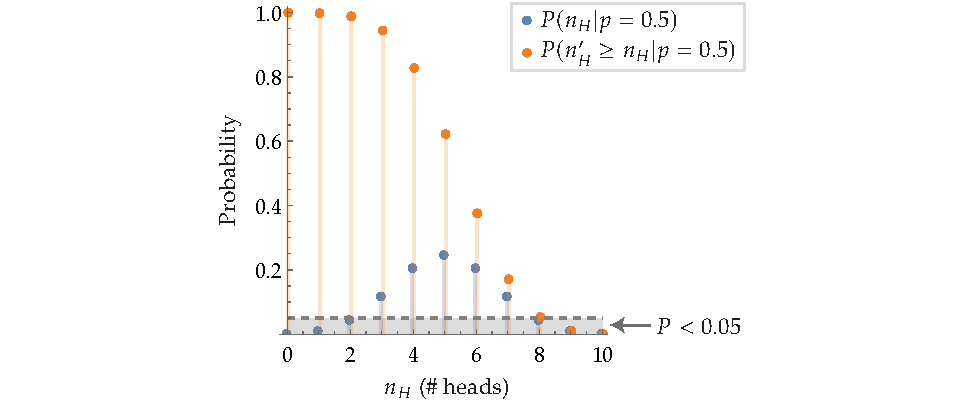
\includegraphics{max_dissertation//chapters//figures//chp1/coin-flip-fair.pdf}
    \caption{Distribution of the number of heads~$n_H$ observed over ~$n = 10$ flips of a fair coin and the resulting p-value probabilities of observing at least~$n_H$ heads. The region where the p-value is less than 0.05 is plotted in gray, a threshold to reject the null hypothesis of a fair coin.}
    \label{fig:coin-flip-fair}
\end{figure}

A smaller p-value yields a more \emph{statistically significant} rejection of the null hypothesis. A threshold of~$P < 0.05$ is often used as a minimum standard, in which case we would reject the hypothesis of a fair coin in our experiment if 9 or 10 of the coin flips land heads. This demarcation at $0.05$ is arbitrary; however small there is always some chance that a genuine fair coin produced an observation as unusual as the one made. We would expect to obtain a p-value less than 0.05 and so reject the model in 1 of 20 experiments conducted with even a truly fair coin. The choice of p-value threshold reflects a tolerance for this possibility that our rejection is the result of chance rather than a genuine signal. 

If such significance testing has led us to doubt that the coin is fair, we may consider an alternative hypothesis. We could instead model a biased coin whose flips are still independent but land heads with some fixed probability~$p \in [0,1]$ and tails with probability~$1 - p$. Under this assumption the likelihood of a sequence with~$n_\text{H}$ heads and~$n_\text{T} = n - n_\text{H}$ tails is \begin{align}
P(\overbrace{\text{H},...,\text{T}}^{n_\text{H} \text{ heads}}|p) = p^{n_\text{H}}(1-p)^{n - n_\text{H}}. \label{eq:coin-flip-likelihood}
\end{align}
This defines a \emph{nested model} by generalizing the fair coin as the special case~$p = 0.5$. Thus the original fair coin model can be directly compared against other choices of the \emph{parameter}~$p$ which each represent possible coins of varying levels of bias towards landing heads or tails. Before the experiment begins we imagine all these coins are possible and aim to \emph{infer} the "true" value of~$p$ realized by our coin based on the observations.

To apply this model suppose that after 10 trials we observe a sequence \begin{align}
    (\text{H}, \text{H}, \text{T}, \text{T}, \text{H}, \text{T}, \text{T}, \text{H}, \text{T}, \text{T}), \label{eq:coin-flip-observations}
\end{align}
now a mixture of~$n_\text{H} = 4$ heads and~$n_{\text{T}} = 6$ tails. We fit the model likelihood Eq.~\eqref{eq:coin-flip-likelihood} to this data by finding the value of~$p$ which would maximize the probability that our observed sequence occurred. For this model this is simply equal to the observed fraction of heads \begin{align}
    \hat{p}_{\text{ML}} = \frac{n_\text{H}}{n}
\end{align} where the "ML" subscript indicates that this is the \emph{maximum likelihood} estimate of~$p$. Our sequence of observations \eqref{eq:coin-flip-observations} gives the estimate~$\hat{p}_{\text{ML}} = 0.4$. 

Although this~$\hat{p}_{\text{ML}}$ is the single parameter value most likely to have generated our observations, it is unclear how seriously we should take the estimate. If the coin was in fact fair,~$p = 0.5$, the slight imbalance towards tails we observe could very well be a random fluctuation in our small sample size as seen in Figure~\ref{fig:coin-flip-fair}. In our earlier language the p-value is not small enough to warrant rejecting the null hypothesis of a fair coin. To conclude that the one "true" value of~$p$ is 0.4, for example to predict that 400 of the next 1000 flips will be heads, would likely~\emph{overfit} the data. As a more extreme example if we only observe a single coin flip which happens to land heads, the maximum likelihood estimate would conclude that~$\hat{p}_{\text{ML}} = 1$ and thus that the coin will always land heads. There should be uncertainty in our conclusions, particularly when they are based on such little evidence. 

By adopting a \emph{Bayesian} perspective we can naturally represent this uncertainty in our inferences. In this framework we critically never exclude the possibility of any potential parameter value. Rather we infer from the data that some parameter values are more probable than others. At each stage of the experiment we represent our~\emph{belief} of likely values as a distribution over all possibilities rather than a single best-fit point. 

Before considering the data we define a~\emph{prior distribution} (or "prior") over the parameters that reflects our initial assumptions. Depending on the context of our experiment we may have quite different expectations that will rightfully influence the conclusions we draw. For example if we use a standard legal tender coin we may hesitate to conclude that the coin is notably biased, even after observing 10 heads in a row. However, if the flips instead involve either a hypothetical or peculiar-looking coin there may be more room for doubt. The form of the prior distribution precisely specifies our initial assumptions.

For our example we will adopt a prior assumption that the coin is likely to be fair or approximately fair. Although a physical coin could conceivably be as biased as~$p = 0.4$, we expect a balanced~$p = 0.5$ to be far more likely. To represent this we define a prior distribution over possible~$p$ peaked at~$p = 0.5$, particularly a beta distribution~$p \sim B(20,20)$ \begin{align}
    P(p) = \frac{41!}{20!20!} p^{20}(1-p)^{20}, \label{eq:coin-flip-P-p}
\end{align} 
plotted in Figure~\ref{fig:coin-flip-inference}c. This particular form of the prior and the number 20 are arbitrarily chosen for this example, although they represent a reasonable assumption for this scenario. 

\begin{figure}
    \centering
    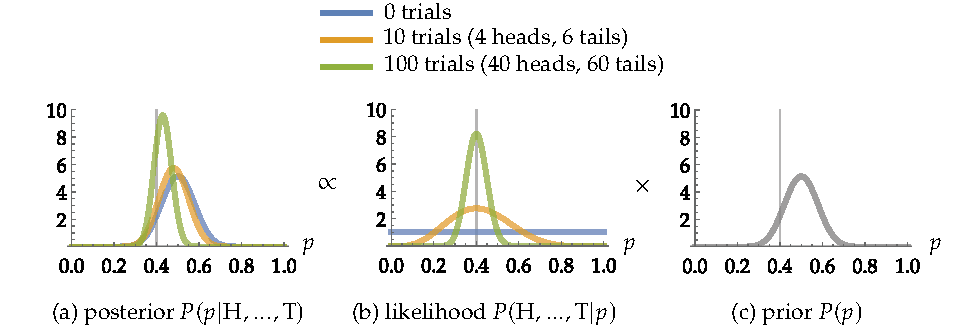
\includegraphics{max_dissertation//chapters//figures//chp1/coin-flip-inference.pdf}
    \caption{(a) Posterior distributions of the parameter~$p$ after observing 0 coin flips (a.k.a. prior distribution), 10, and 100 coin flips. In each experiment~40\% of trials are heads, a ratio marked by the vertical line in each plot. The posterior distributions are proportional to the product of the likelihood (b) and prior (c) over~$p$. As more observations are made the posterior is increasingly informed by the model likelihood.}
    \label{fig:coin-flip-inference}
\end{figure}

As we observe coin flips we update these prior beliefs to reflect new data and arrive at a new \emph{posterior} distribution of likely parameter values. Using Bayes' law this posterior distribution is proportional to the product of the model likelihood and the initial prior distribution as \begin{align}
    P(p|\text{H},...,\text{T}) \propto P(\text{H},...,\text{T}|p)P(p). \label{eq:bayes-law-prop}
\end{align}
This form ensures that when no data is observed the posterior distribution is equal to the prior assumption~$P(p)$. As flips are recorded the influence of the prior distribution wanes as the posterior is dominated by the model likelihood~$P(\text{H},...,\text{T}|p)$. Figure~\ref{fig:coin-flip-inference} demonstrates this shift in the posterior distribution (a) from the prior (c) to the likelihood (b) after making 0, 10, and 100 observations at a ratio of 40\% heads. As more observations are made with an empirical probability of~$p = 0.4$, our posterior distribution becomes increasingly concentrated around that belief. We must however observe sufficient evidence to overcome the strength of our initial assumptions before coming to that conclusion with certainty.

The width and form of the posterior distribution gives a full picture of the uncertainty of our the inference. Although the posterior distribution in Figure~\ref{fig:coin-flip-inference}a after observing 100 flips is tightly concentrated around a probability~$p \sim 0.4$, we retain some ambiguity if the parameter might deviate slightly from that peak. Nonetheless it is often useful to report the single choice of parameter most favored by the posterior distribution, known as the \emph{maximum a posteriori} (MAP) estimate. For our example and choice of prior Eq.~\eqref{eq:coin-flip-P-p} this is \begin{align}
    \hat{p}_{\text{MAP}} = \frac{n_H + 20}{n + 40}. \label{eq:coin-flip-p-MAP}
\end{align}
The earlier interplay between the prior and likelihood is present in this estimate. When no coin flips are observed we obtain the prior assumption~$\hat{p}_{\text{MAP}} = 0.5$. As the number of observations~$n$ increases, this Bayesian estimate approaches the frequentist maximum likelihood estimate, $\hat{p}_{\text{MAP}} \rightarrow \frac{n_H}{n} = \hat{p}_{\text{ML}}$. 

To complete Bayes' law and fully specify the posterior distribution we normalize Eq.~\eqref{eq:bayes-law-prop} as 
\begin{align}
    P(p|\text{H},...,\text{T}) &= \frac{P(\text{H},...,\text{T}|p)P(p)}{P(\text{H},...,\text{T})} \label{eq:bayes-law} 
\end{align}
where \begin{align}
    P(\text{H},...,\text{T}) = \int_0^1 P(\text{H},...,\text{T}|p)P(p) dp
\end{align}
is the \emph{evidence} (or "marginal likelihood") of the model. This evidence can be interpreted as the probability of arriving at the observations~$\text{H},...,\text{T}$ through the two stage process of first choosing a parameter~$p$ from the prior~$P(p)$ then generating the data from the model likelihood~$P(\text{H},...,\text{T}|p)$. By integrating over all possible parameters~$p$, the Bayesian evidence is equal to the total probability that a model generates the observed data from our prior assumptions. A cartoon of this generative process is given in Figure~\ref{fig:bayesian-evidence}.

\begin{figure}
    \centering
    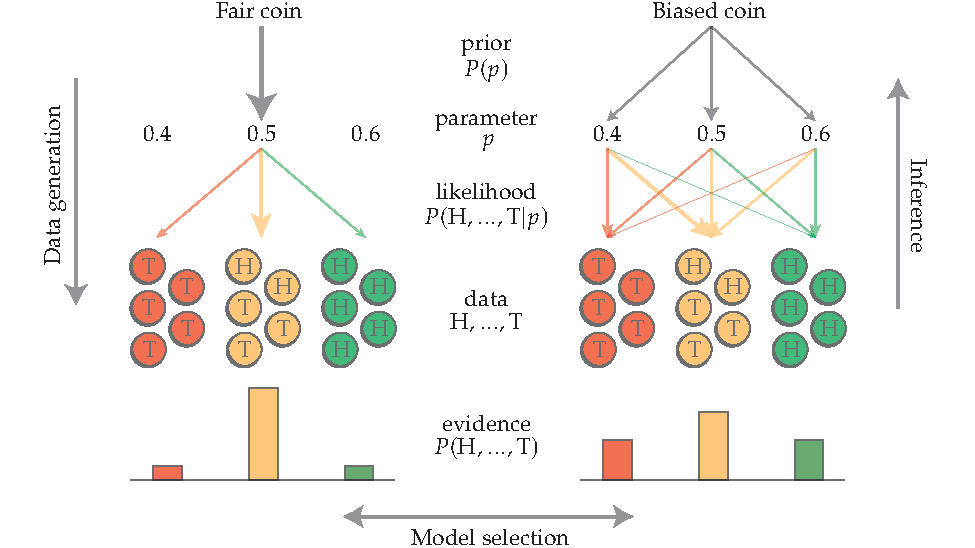
\includegraphics{max_dissertation//chapters//figures//chp1/bayesian-evidence.pdf}
    \caption{Schematic of the full generative process of the fair and biased coin models. A parameter value~$p$ is first drawn from the appropriate prior~$P(p)$, represented by the thicknesses of the top gray arrows to example parameter values~$p = 0.4, 0.5,$ and $0.6$. The data is drawn from the model likelihood~$P(\text{H},...,\text{T}|p)$ given that parameter. Examples of the likelihood of three potential sequences of all tails, all heads, and a mixture are indicated by the weights of the colored arrows. Lastly the probability of all generative paths leading to a given observation sum to the model evidence. The evidence of the two models is then used to select between the models given an observation. }
    \label{fig:bayesian-evidence}
\end{figure}

This is a useful interpretation for comparing competing models of a data set to perform \emph{model selection}. A model with higher Bayesian evidence is more likely to have produced the observed data, and therefore has reason to be preferred. As an application we can compare the strict fair coin model described in Eq.~\eqref{eq:coin-flip-fair-likelihood} to the Bayesian model with the more permissive prior Eq.~\eqref{eq:coin-flip-P-p} on the observations~\eqref{eq:coin-flip-observations} of 4 out of 10 heads. The fair coin model assumes that the coin is exactly fair regardless of the observed evidence, an assumption that can be represented with a Dirac delta function prior \begin{align}
    P_{\text{fair}}(p) &= \delta(p - 0.5).
\end{align}
In this case integrating over the prior simply evaluates at~$p = 0.5$ to give the model evidence \begin{align}
    P_{\text{fair}}(\text{H},...,\text{T}) = \int_0^1 P(\text{H},...,\text{T}|p)P_{\text{fair}}(p) dp = \frac{1}{2^n} \approx 0.097\%
\end{align}
that the fair coin model would generate our sequence. In comparison the model evidence with the prior Eq.~\eqref{eq:coin-flip-P-p} is \begin{align}
    P_{\text{gen}}(\text{H},...,\text{T}) = \int_0^1 P(\text{H},...,\text{T}|p)P(p) dp = \frac{41!(20+n_H)!(20+n_T)!}{(41 + n)!20!20!} \approx 0.091\%,
\end{align}
and so this more general model is overall (slightly) less likely to have generated our observations. The ratio of such evidences is known as a \emph{Bayes factor} between the two models, in this case the ratio \begin{align}
    \frac{P_{\text{gen}}(\overbrace{\text{H},...,\text{T}}^{10 \text{ flips}})}{P_{\text{fair}}(\text{H},...,\text{T})} \approx 0.93
\end{align}
less than 1 indicates that the more complex model is not justified over the fair coin. We note here that the Bayesian evidence has naturally penalized over-parametrization. Although the choice of parameter~$p = 0.4$ does a better job than the fair coin in isolation, it has a higher model likelihood, this peak must be weighed against all possible other values of the parameter which in this case offset that advantage.

Had we instead observed 40 heads out of 100 flips, the Bayes factor flips to \begin{align}
    \frac{P_{\text{gen}}(\overbrace{\text{H},...,\text{T}}^{100 \text{ flips}})}{P_{\text{fair}}(\text{H},...,\text{T})} \approx 2.25 \label{eq:coin-flip-bayes-factor}
\end{align}
as the more flexible model is now preferred in the presence of increased evidence that the coin is not quite fair. Depending on the particular data set being considered we may prefer one model or the other. 

In fact, given two models~$M_1$ and~$M_2$, there will always be data sets that prefer one model over the other. No model can be strictly better than another across all possible observations. To see this, consider the Bayesian evidences~$P_1(\vec{s})$ and~$P_2(\vec{s})$ of the two models. Both of these are normalized distributions over the possible observations that a model can generate. If we assume that the Bayesian evidence~$P_1(\vec{s})$ is greater than~$P_2(\vec{s})$ for any observation~$\vec{s}$, both distributions can not be simultaneously normalized to 1 as \begin{align}
    1 = \sum_{\vec{s}} P_1(\vec{s}) > \sum_{\vec{s}} P_2(\vec{s}) \not= 1.
\end{align}
Therefore both an observation~$\vec{s}_1$ that favors model 1 and an observation~$\vec{s}_2$ that favors model 2. In this spirit this inherent trade-off is sometimes known as the "no free lunch" theorem~\cite{Peixoto17}. When building models and performing model selection between them, we hope that "realistic data sets" fall within the preferred domain of our models. 

When considering a data set, we can also compute Bayes factors like Eq.~\eqref{eq:coin-flip-bayes-factor} by taking advantage of the nested structure of our model. Since the general model is equivalent to the fair coin model at the value~$p = 0.5$, the Bayes factor can be written in terms of the posterior distribution at that value. Here we have \begin{align}
    P(p = 0.5|\text{H},...,\text{T}) = \frac{P(\text{H},...,\text{T}|p = 0.5)P(p = 0.5)}{P(\text{H},...,\text{T})} = \frac{P_{\text{fair}}(\text{H},...,\text{T})}{P_{\text{gen}}(\text{H},...,\text{T})}.
\end{align}
Because of this, if our posterior distribution in the general model is meaningfully peaked at~$p = 0.5$, the evidence of the fair coin is greater than that of the general coin. If the posterior excludes~$p = 0.5$, the reverse is true. 

This formulation is useful since it is in practice often difficult to compute the absolute Bayesian evidence of a model since it involves integrating over the high dimensional space of all possible parameter values. If we define a nested model, however, we can approximate the posterior distribution using Monte Carlo methods discussed in Section~\ref{app:statistical-physics} relatively easily to and so compute these Bayes factors and compare models. 

We apply this central trick to a range of cases across Chapters~\ref{chp:group-structure} and~\ref{chp:hierarchies}. In each example we start with a simple model then generalize it within this Bayesian framework. By doing this we can check both whether this generalization is warranted and, if so, measure the size of the new effect, just like we infer~$p$ in the biased coin model. By stating and incorporating our prior expectations into the inference process, a Bayesian framework enables us to handle uncertainty and validate our models in a graceful manner.